\chapter{Arquitetura do \textit{middleware} de comunicação}

Este capítulo descreve em detalhes a arquitetura do proposto \textit{middleware} de comunicação, tais como suas partes e suas principais funções, como troca de mensagens, migração e serialização. 

\section{Componentes do \textit{middleware}}

A arquitetura proposta é dividida em dois componentes principais: o ambiente (\textit{envinonment}) e o processo lógico (\textit{process}). Um ambiente representa um nó lógico do sistema de simulação distribuída, ou seja, é a representação lógica de um computador no sistema distribuído. Em uma simulação distribuída, tipicamente, cada nó físico da rede deve conter um único \textit{environment}.

O segundo componente da estrutura do \textit{middleware}, o processo lógico, que é a representação lógica de um processo no sistema de simulação distribuída. Na arquitetura aqui descrita, um processo lógico somente existe dentro de um \textit{environment}. Sendo assim, um \textit{environment} pode ser visto como um conjunto de processos. Por sua vez, um processo somente pode estar contido por um único \textit{environment} em um determinado momento.

Assim, sendo \textit{p} um processo lógico e \textit{e} um ambiente de simulação contento \textit{n} processos, então definimos:

Definição 1: Um \textit{environment} é um conjunto de processos \begin{equation} e_{k} = \{p_{i} | i < n \} \end{equation}

Definição 2: Um processo só pode estar contido em um único ambiente em um instante bem definido \begin{equation} p_{k} \in e_{l} \rightarrow \not \exists e_{m}, p_{k} \in e_{m}, e_{l} \neq e_{m} \end{equation} 

Tanto o \textit{environment} quanto o \textit{process} são abstrações lógicas que representam a simulação baseado em eventos discretos. Fisicamente tanto o ambiente quanto o processo lógico são instâncias de objetos que devem ser implementadas extendendo classes bases abstratas que contém as especificações descritas por este \textit{middleware}.

A arquitetura do \textit{middleware} aqui proposto deve oferecer as seguintes funcionalidades:
 
\begin{itemize}
\item Comunicação entre processos lógicos por troca de mensagens.
\item Serialização do conteúde de um processo lógico.
\item Migração de um processo de um \textit{environment} para outro.
\item Continuidade da comunicação, de maneira transparente, mesmo após a migração de um processo.
\item Serialização em larga escala de um ambiente ou de toda a simulação.
\item Comunicação grupal entre processos e entre ambientes.
\end{itemize}

A propriedade de comunicação por troca de mensagem é um ítem fundamental para a implementação de simulação distribuída. A forma de se comunicar por troca de mensagens provida pelo \textit{middleware} baseia-se nas quatro suposições iniciais descritas por \cite{MCQUILLAN75} sobre os canais de comunicação inter-processos:

\begin{itemize}
\item O canal introduz um flutuante, porém finito, atraso nas mensagens.
\item O canal possui uma flutuante, porém finita, largura de banda.
\item O canal apresenta uma flutuante, porém finita, taxa de erro.
\item Existe uma real possibilidade de as mensagens transmitidas da fonte para o destino cheguem ao destino em uma ordem diferente da originalmente transmitida. É assumido que tanto a fonte quanto o destino possuem, em geral, finitos tamanhos de \textit{buffers} de armazenamento e diferentes \textit{bandwidth}.
\end{itemize}

A capacidade de um processo lógico migrar de um \textit{environment} para outro é um ponto fundamental para se proporcionar a capacidade de balanceamento de cargas em uma simulação distribuída. O mecanismo de migração, descrito na Seção~\ref{migracao}, é a união da capacidade de serialização de um processo e da comunicação entre diferentes \textit{environments}.

\section{O componente \textit{environment}}

Essencialmente, um ambiente na arquitetura aqui proposta é uma plataforma que abriga e gerencia diversos processos lógicos. A existência desta plataforma como base para o gerenciamento dos processos é justificada quando desejamos manipular simultaneamente características de diversos processos que possuêm em comum o fato de estarem no mesmo ambiente físico (como por exemplo migrar ou serializar todos os processos). Mas principalmente se justifica a existência de uma camada que seja responsável por gerenciar o ciclo de vida de processos, como criação, migração e destruição de processos.

\subsection{Estrutura interna}

Internamente, o \textit{environment} apresenta as seguintes estruturas básicas (conforme ilustrada na Figura~\ref{fig:environment_1}):

\begin{itemize}
\item Estrutura interna de dados do ambiente
\item Tabela de endereços de processos
\item Lista de processos lógicos locais
\item Proxy de comunicação externa
\end{itemize}

\begin{figure}
  \centerline{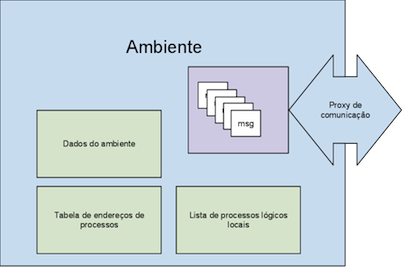
\includegraphics{Environment_1.png}}
  \caption{A arquitetura interna de um \textit{environment}.}
\label{fig:environment_1}
\end{figure}

A estrutura interna de dados do ambiente é a representação de todos as variáveis pertencentes ao \textit{environment}. Dados como o endereço físico (IP) do ambiente na rede, nome lógico do ambiente e quantidade de processos residentes no \textit{environment} são armazenadas neste espaço.

Um \textit{environment} possui um endereço lógico único em toda o ciclo de vida da simulação, denominado \textit{Unique Environment Identifier} - \textit{UEI}. Este endereço é um número natural que o representa no sistema de simulação.

A comunicação entre dois \textit{environmets} se dá através seu endereço físico na rede. Tal inflexibilidade é justificada quando assumimos que um \textit{environment} tem todo o seu ciclo de vida atrelado a uma mesma máquina física (salvo excessões descritas na Seção~\ref{migra_ambiente})

\subsection{\textit{Proxy}}

O \textit{proxy} é a camada do \textit{environment} que é responsável por toda troca de mensagem entre os processos. O \textit{proxy} atua de maneira distinta em troca de mensagens entre processos que convivem no mesmo ambiente e entre trocas de mensagens entre processos que se situam em ambientes distintos. As distinções entre trocas de mensagens internas e externas serão tratadas na seção~\ref{troca_mensagens}

O \textit{proxy} também é o único canal por onde os processos recebem mensagens providas de fora do ambiente. Toda mensagem recebida pelo proxy é identificada pelo noem lógico do processo destinatário. Cabe ao proxy converter este nome lógico em seu endereço físico e encaminhar a mensagem ao processo de destino.

Como todo o tratamento de envio e recebimento de mensagens deve ser não-blocante, este componente deveoperar de maneeira assíncrona aos demais componentes do \textit{environment}. De maneira análoga, pode se dizer que o \textit{proxy} é um subprocesso executando deentro do processo físico \textit{environment}.

\subsection{Tabela de endereços de processos}

A tabela de endereços dos processos é uma lista associativa que possui informações básicas de endereços e status dos processos existentes. Esta tabela contém informações não apenas dos processos residentes no \textit{environment} em questão, mas sim dados de todos os processos existentes na simulação (mesmo que desatualizados, dependendo do instante). Dados referentes aos processos residentes no mesmo \textit{environment} da tabela de endereço de processos estarão, invariavelmente, atualizados.

Conforme previamente mencionado, para realizar a comunicação entre processos é utilizado como identificador do processo não o seu endereço físico, mas sim seu endereço lógico no sistema. O motivo de se utilizar o endereço lógico é que este, ao contrário do endereço físico, é único em todo o ciclo de vida do processo. Isto garante que após uma migração de um environment para outro, um processo possa continuar a ser encontrado pelo mesmo endereço lógico (o que não aconteceria caso o endereço físico fosse usado, uma vez que após uma migração o endereço de IP do environment, e a porta a qual o processo está vinculado, sofreriam variações). Esta característica de ser identificado sempre pelo mesmo endereço lógico é fundamental para evitar a constante alteração de dados referentes aos processos em inúmeras partes do sistema.

Além de armazenar dados refrente aos endereços lógicos e físicos dos processos, a tabela de endereços armazena também uma variável de \textit{status} de cada processo. Os estados de um processo podem ser:

\begin{itemize}
\item Ativo: Indica que o processo se encontra neste \textit{environment} e está ativo. 
\item Ausente: Indica que o processo em questão se encontra em outro ambiente.
\item Trânsito: Indica que o processo em questão estava em um momento anterior neste ambiente e foi migrado para um ambiente diferente, porém ainda não atualizou a tabela de endereços com seu endereço atual.
\item Inativo: Indica que o processo se encontra neste ambiente, mas não está ativo.
\end{itemize}

Os estados ativo e inativo são os estados mais comuns de um processo em um sistema típico. Eles indicam que o processo em questão está, ou não, em execução naquele ambiente. Um processo em estado inativo significa que este está residente no \textit{environment} em questão, mas não está executando no momento por algum motivo não identificado. Toda mensagem recebida para ser entregue a um processo inativo será armazenada no buffer de mensagens do \textit{proxy} e deverá ser retirada posteriormente pelo processo.

O estado de trânsito indica que o processo esteve naquele \textit{environment} em algum instante do passado e que sofreu uma migração, mas seu novo endereço não foi ainda atualizado. Mais informações de como funciona a atualização de endereços durante a migração pode ser encontrado na Seção~\ref{atualizacao}.

\section{O componente \textit{process} \label{process}}

Um processo é uma unidade discreta de processamento em um sistema de simulação de eventos discretos. É ele o responsável por retirar cada evento a ser executado da fila de eventos futuros e executá-lo. A representação de um processo lógico na arquitetura aqui descrita se dá pelo objeto \textit{process}. Este deve ser capaz de abrigar componentes que descrevem o comportamento do sistema a ser simulado, apoiando-se nos mecanismos de troca de mensagens, serialização e locomoção (migração) de processos providos pelo \textit{environment}.

Um processo lógico possui três identificações distintas no sistema: seu endereço físico em memória, seu endereço físico na rede e seu endereço lógico no sistema de simulação. Na arquitetura deste \textit{middleware}, o processo é referenciado para troca de mensagens ou por seu endereço físico na rede, ou por seu endereço lógico no sistema de simulação. A distinção se a comunicação é feita através do endereço físico ou lógico se dá a partir de qual nível da arquitetura se dá a comunicação ().

Como uma das premissas do \textit{middleware} de comunicação é tratar de maneira completamente transparente para o usuário a comunicação entre os processos, o mecanismo de troca de mensagem entre dois objetos do tipo \textit{Process} deve ser encapsulado e resolvido pelo próprio objeto (em conjunto com o \textit{environment} e seu \textit{proxy}), não transferindo assim ao usuário os encargos da troca de mensagem entre processos.

Neste ponto a comunicação se divide em doi tipos diferentes: comunicação entre processos cohabitantes (que habitam o mesmo \textit{environment}) e comunicação de processos não-cohabitantes (\textit{environment} diferentes). Essa diferença força a utilização de meios distintos de comunicação para cada caso, porém isto é resolvido internamente pelo \textit{middleware}, deixando a comunicaçào transparente para o \textit{framework}.

Desta forma, internamente um processo lógico deve ser capaz de se comunicar com o processo alvo da maneira mais eficiente possível. Assim sendo, é natural que processos que residam em um mesmo \textit{environment} possuam um canal diferenciado de comunicação, ao ponto que processo que estão em ambientes distintos compartilhem canais comuns de comunicação.

Em contrapartida, é justificável que processos que não se comunicam com grande frequência (ou que nunca se comunicam) não tenham conhecimentos uns dos outros. A abstração provida pelo \textit{environment} garante o isolamento entre o endereço físico de um processo e o seu nome lógico no sistema. Este desacoplamento entre endereço lógico e físico de um processo garante também a continuidade da comunicação entre processos lógicos após sua migração. Assim sendo, uma vez que um determinado processo tenha que enviar uma mensagem para um segundo processo, cabe ao \textit{environment} identificar o destinatário da mensagem e a despachar.

Toda comunicação que é iniciada a partir de um processo, é feita através do endereço lógico do processo. Isto garante que o usuário do \textit{middleware} não precise se adentrar em estruturas físicas do sistema, como saber qual o endreço físico (IP:PORT) está o processo com o qual ele deseja se comunicar. Cabe ao \textit{environment} que abriga o remetente da mensagem encaminhá-la para o endereço físico correspondente.

O endereço lógico de um processo é denominado \textit{Unique Process Identifier} - \textit{UPI}. Para garantir que cada processo tenha um endereço lógico único no sistema sem a necessidade de sincronização de todo o sistema em cada criação de um novo processo lógico, a construção deste endereço lógico se dá por uma tupla, onde o primeiro elemento é o \textit{UEI} do \textit{environment} onde este processo foi criado, e o segundo elemento da tupla é um número sequencialmente incrementado pelo ambiente a cada novo processo criado. Isto garante que cada processo possua um par de números único em todo o sistema compondo a sua tupla de identificação.

Vale ressaltar que o \textit{UPI} é único em todo o ciclo de vida de um \textit{process} e, portanto, não se altera em caso de migração. Mesmo após migrar de um ambiente para outro, o primeiro elemento da tupla de identificação continua representando o ambiente onde o processo foi criado pela primeira vez.

Mais detalhes sobre a comunicação entre processos e a distinção entre comunicação entre processos cohabitantes e não-cohabitantes são detalhados na seção~\ref{troca_mensagens}.

\subsection{Ciclo de vida de um processo}

Um processo lógico tal como descrito pelo \textit{middleware} possui um ciclo de vida com fases bem definidas. Isso significa que a classe base a qual o usuário do \textit{middleware} extende para criar seu processo lógico já prevê, na forma de métodos abstratos, \textit{slots} onde serão implementados trechos importantes para fases específicas da vida do processo. Essas fases estão ilustradas no diagrama da Figura~\ref{fig:estados_processos}. A representação dos \textit{slots} onde serão inseridos os códigos, na forma de métodos abstrados é ilustrada na representação UML da Figura~\ref{fig:process_uml}.

O primeiro método invocado automaticamente pelo processo na sua criação é o método on\_create. Este método é chamado apenas uma única vez em todo o ciclo de vida do processo lógico e trata das rotinas de inicialização do processo. Este método pode ser visto de maneira análoga ao construtor de uma classe, na programação orientada a objetos. Imediatamente após executar o código contido no método on\_create, o próximo méto invocado automaticamente pelo sistema é o método run.

O conteúdo do método run é onde o corpo da simulação deve estar implementado. É neste ponto do código onde a a simulação deverá retirar o próximo evento da lista de eventos futuros e executá-lo. Vale ressaltar que como descreve \cite{RIBEIROALVES}, o processo de se retirar eventos da fila de eventos futuros para execução não pode se dar na forma de um laço de repetição, pois tornaria a execução do método run não-preemptiva. A solução apontada por \cite{RIBEIROALVES} é a de, após realizar a execução de um ítem da fila de eventos futuros, enviar uma mensagem para si mesmo agendando a execução do evento seguinte. Isto garante a preempção da simulação para tratamento de mensagens externas, migrações, etc.

\begin{figure}
  \centerline{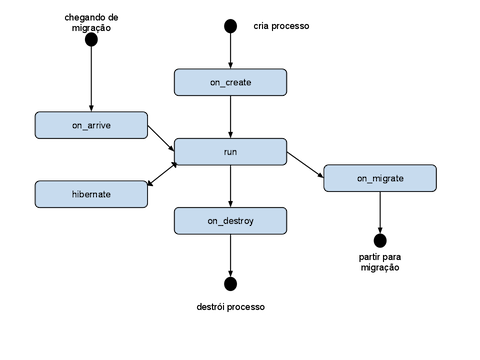
\includegraphics{estados_processos.png}}
  \caption{Ciclo de vida de um processo lógico.}
\label{fig:estados_processos}
\end{figure}

\begin{figure}
  \centerline{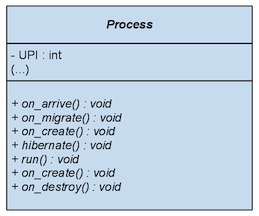
\includegraphics{process_uml.png}}
  \caption{Representação em diagrama de classe do componente \textit{process}.}
\label{fig:process_uml}
\end{figure}

Os demais métodos invocados automaticamente pelo sistema são on\_migrate, invocado antes da migração. on\_arrive, invocado assim que o processo chega no destino. hibernate, invocado quando um processo é adormecido e on\_destroy, invocado ao se destruir um processo lógico.

Naturalmente o a classe \textit{Process} comporta a criação de demais métodos além destes pré-estipulados, porém apenas estes métodos são executados de maneira automática pelo \textit{middleware} em ocasiões especiais.

\subsection{Serialização de um processo}

Serialização é a capacidade que um objeto possui de converter sua estrutura interna de dados em um formato estático, a fim de se armazenar ou reutilizar posteriormente

Um processo deve possuir a propriedade de ser serializado quando conveniente. Um processo não possui a capacidade de se serializar, ou de serializar um outro processo. O processo de serialização de um processo se dá somente a partir de chamadas internas do \textit{middleware}. Ao usuário cabe garantir que todo o código escrito seja serializável.

\section{Migração de processos \label{migracao}}

Uma das principais características propostas pelo \textit{middleware} de comunicação que compões este trabalho á a possibilidade de que processos lógicos migrem de seu nó de origem para um nó distinto no sistema. Para que isso ocorra, naturalmente, o nó destinoo deve possuir uma instância ativa de um \textit{environment} capaz de gerenciar a continuidade da vida do processo em questão.

Para que a migração ocorra, uma série de ações deve ocorrer a fim de sinalizar 

\begin{enumerate}
\item O estado do processo na tabela de endereços é modificade de Ativo para Trânsito.
\item O método on\_migrate é invocado ainda no ambiente de origem do processo.
\item O processo a ser migrado é serializado pelo \textit{environment} de origem e enviado para o ambiente de destino.
\item O ambiente de destino recebe o processo serializado e o desserializa, tornando-o um novo objeto em memória, mas mantendo os dados originais do processo.
\item O ambiente de destino atualiza o estado do processo em sua tabela local de Ausente para Inativo.
\item O ambiente de destino envia uma mensagem para o ambiente de origem indicando que o processo chegou, e qual o novo endereço físico do processo.
\item O \textit{environment} de origem atualiza o estado do processo para Ausente. Atualiza também o endereço físico do processo na tabela de endereços.
\item O processo executa o método on\_arrive no ambiente de destino.
\item O \textit{environment} muda o status do processo de Inativo para Ativo.
\item Por fim, o processo recupera todas as mensagens do buffer de mensagens do proxy de comunicação, resgatando eventuais mensagens recebidas enquanto o seu estado era Inativo.
\item O processo, já em estado ativo, executa o método run.
\item Uma mensagem em \textit{broadcast} é enviado a todos os \textit{environment}, sinalizando o novo endereço físico correspondente à aquele processo acaba de migrar. As tabelas de endereços são então atualizadas.
\end{enumerate}

Assim que o processo termina o ciclo de ações de migração ele está apto a continuar a simulação do ponto onde parou no ambiente antigo. Isto se dá poque o processo foi serializado e todos os dados foram mantidos tais como estavam instantes antes da migração.

Vale ressaltar que uma vez que esteja em processamento (executando o método run), o processo só executa a migração após o término da execução do evento em questão. Sendo assim, o método run deve ser implementado de maneira a possibilitar a preempção de eventos.

\subsection{Atualização da tabela de endereços dos processos \label{atualizacao}}

Uma vez que um processe migra de um \textit{environment} para outro, instantes após a migração apenas os dois ambientes envolvidos possuem os dados atualizados. Todo ambiente difente dos envolvidos no processo de migração possuem em suas tabelas de endereços de processos dados incorretos quanto a sua localização, portanto, enviariam mensagens para o ambiente antigo, ao qual o processo destinatário não mais pertence.

Ao receber uma mensagem de um antigo hospedeiro, um \textit{environment} (que possui o seu novo endereço), redireciona a mensagem ao proxy do ambiente que possui atualmente o processo em questão. Porém, isso inclui mais um intermediário no processo de transmissão de mensagens. Sendo assim, duas ações, em momentos distintos, são efetuadas para garantir a atualização das tabelas de endereços de processos. Primeiro, o antigo \textit{host} do processo, ao receber a mensagem, al;em de repassa-la ao atual \textit{host} também devolve uma mensagem para o remetente da mensagem, notificando-o que o endereço do ambiente que contém o processo mudou, e atualiza este endereço.

Em um momento distinto, uma segunda ação de sincronismo de tabelas é disparada. Esta ação é iniciada de forma idependente por cada \textit{environment}, enviando uma mensagem para os demais ambientes, notificando-os de quais processos lógicos encontram-se em seu poder. Isto garante uma atualização constante das diversas tabelas de endereços de processos existente na simulação.

\section{Troca de mensagens \label{troca_mensagens}}

No modelo de comunicação baseado em proxy, quando um processo deseja enviar uma mensagem a um segundo processo, a mensagem é primeiramente enviada ao proxy do \textit{environment} ao qual o processo remetente reside, e o proxy é responsável por resolver a correlação entre endereço lógico e o endereço físico, e enfim enviar a mensagem ao processo destinatário. O principal motivo de se deixar o proxy responsável pelo envio da mensage é se possibilitar que existam uma pequena quantidade de tabelas de correlação de endereços, e assim, que existam menos atualizações de tabelas em uma migração.

Em um modelo onde cada processo resolveria o envio de mensagem diretamente, a quantidade de tabelas de endereços seria proporcional à quantidade de processos (e não proporcional à quantidade de ambientes, como é na arquitetura proposta). Ao haver uma migração, existirão menos tabelas a serem atualizadas na arquitetura baseada em comunicação inter-proxies, ao passo que na comunicação direta entre processos, a quantidade de tabelas a serem atualizadas seria bem maior.

\subsection{Comunicação direta e indireta}

Quando a comunicação é feita por dois processos lógicos residentes em diferentes \textit{environments} (e por consequência, em máquinas distintas da rede) a comunicação se passa através do \textit{proxy} do \textit{environment} do remetente, e esse é responsável por enviar a mensagem ao \textit{proxy} do processo destinatário. O fluxo de comunicação é ilustrada de maneira simplificada na Figura~\ref{fig:indireta}.

Neste caso, quando ao processo P1 enviar uma mensagem ao processo P3, o próprio processo requisita diretamente ao \textit{environment} o envio da mensagem. A mensagem é então encaminha de P1 para o \textit{proxy} do seu \textit{environment} que detecta, através da tabela de endereço de processos, o endereço físico do processo alvo. 

Uma vez que a mensagem a ser enviada está em posse do \textit{proxy} do \textit{environment} destinatário, duas modalidades de comunicação podem ocorrer. A modalidade padrão é a comunicação indireta, onde o \textit{proxy} em posse da mensagem irá envia-la ao \textit{proxy} do ambiente que contém o receptor da mensagem. Uma vez que a mensagem esteja no \textit{proxy} do destinatário, este a encaminha para o processo (Figura~\ref{fig:indireta}).

Uma alternativa à comunicaçào indireta é a comunicação direta, onde o \textit{proxy} do processo de origem, uma vez obtido o endereço físico do processo destinatário, envia a mensagem diretamente para o processo receptor (Figura~\ref{fig:direta}). O método direto é útil por eliminar um intermediário na transmissão da mensagem, mas possui um inconveniente que pode anular o ganho da eliminação do intermediário. Caso haja uma migração, a mensagem não é automaticamente redirecionada para o novo ambiente em que o processo se localiza, mas sim é levantado uma excessão na comunicação, o que levaria a um tratamento de excessão, que por sua vez seria encarregado de localizar o processo em seu novo endereço físico e retransmitir a mensagem.

Cabe salientar que em caso de falha na transmissão da mensagem na modalidade de comunicação direta, a excessão levantada deve ser tratada não pelo processo, mas pelo \textit{environment}, pois a mensagem encontra-se em posse do \textit{proxy}

\begin{figure}
  \centerline{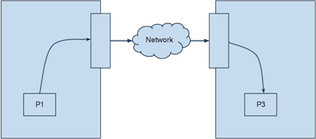
\includegraphics{Communication_indireta.png}}
  \caption{Comunicação indireta \textit{proxy-process}.}
\label{fig:indireta}
\end{figure}

\begin{figure}
  \centerline{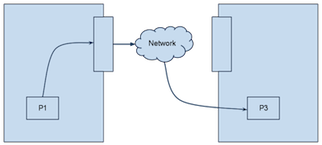
\includegraphics{Communication_direta.png}}
  \caption{Comunicação direta \textit{proxy-process}.}
\label{fig:direta}
\end{figure}

\subsection{Comunicação local direta}

Uma terceira modalidade de comunicação é a comunicação direta, via endereço físico (Figura~\ref{fig:direta_mesmo}), entre processos que habitam um mesmo ambiente. Nesta modalidade um processo que se comunica constantemente com outro processo no mesmo \textit{environment} adquire o seu endereço físico e faz a comunicação direta, sem a necessidade de se passar por um \textit{proxy} de comunicação.

Assim como na comunicação direta, neste caso há um ganho na transmissão da mensagem entre origem e destino por se excluir o \textit{proxy} como intermediário da transmissão. Entretanto, no caso de uma migração, as mensagens não seriam automaticamente redirecionadas para o processo destinatário, cabendo assim ao usuário do \textit{middleware} o tratamento de excessão caso esta aconteça.

A comunicação local direta, assim como a comunicação direta, são opções que devem ser exploradas em casos onde a migração de processos é reduzida ou nula.

\begin{figure}
  %\centerline{\includegraphics{Communication_superdirect.png}}
  \caption{Comunicação direta \textit{process-process}.}
\label{fig:direta_mesmo}
\end{figure}

\section{Serialização em grande escala} %trata da serialização de um environment ou até mesmo da simulação como um todo
\section{Comunicação grupal} % mensagens em multicast
\section{Migraçoes em grande escala e migrações de ambientes \label{migra_ambiente}} %casos de excessão
